\section{Supervised topics with ideal point text regression}

We can generalize ridge regression on ideal points to provide a fully
supervised topic model.  Recall that ridge regression on ideal points
corresponds to the model
\begin{enumerate}
  \item Fit the ideal point model \[
    \label{item:ideal_point}
    \arg \max_{a_d, b_d, x_u} \sum_{u \in U, d \in D} \log p(v_{ud} | a_d, b_d, x_u)
    - \sum_{d \in D} (\lambda_1 a_d^T a_d + \lambda_2 b_d^T b_d)
    - \sum_{u \in U} \lambda_3 x_u^T x_u, \]
    where $p(v_{ud} | a_d, b_d, x_u)$ is the logistic function $\sigma(a_d^T x_u + b_d)$
%    \footnote= \frac{1_{v_{ud} = yea} \exp(a_d^T x_u + b_d) + 1_{v_{ud} = nay}}{\exp(a_d^T x_u + b_d) + 1}
%    \]
    and $\lambda_1, \lambda_2, \lambda_3$ are regularization
    parameters.
  \item Fit the ridge regression
    \label{item:fit_regression}
    \begin{eqnarray*}
      \beta_a, \beta_b \sim N(0, 1 / \lambda_4), \\
    a_d \sim N(\bm w_d^T \beta_a, \sigma_a), \\
    b_d \sim N(\bm w_d^T \beta_b, \sigma_b),
    \end{eqnarray*}
    where $\bm w_d$ are word counts and $\lambda_4$ is a ridge penalty.
\end{enumerate}
Although this model performed well in the prediction task, it suffers
from a critical limitation: the ideal points are informed only by
votes.  The regression coefficients $\beta_a, \beta_b$ are
interpretable, but only in the sense that they relate words to ideal
points.

\paragraph{Ideal point text regression} We can solve this problem by
forcing $\sigma_a, \sigma_b \rightarrow 0$.  We can accomplish this by
modeling the document parameters only implicitly:
\begin{eqnarray}
    \label{item:ideal_point}
    \arg \max_{\bm B, \bm b, x_u} \sum_{u \in U, d \in D} \log p(v_{ud} | \bm w_d, \bm B, \bm b, x_u) - \lambda_1 \sum_{ij} \bm B_{ij}^2 - \lambda_2 x_u^T x_u - \lambda_3 \bm b^T \bm b,
\end{eqnarray}
where $\bm B$ is a $r \times V$ matrix, $x_u$ is again the $r \times 1$
user ideal point, $\bm b$ is a $V \times 1$ vector, $\lambda_i$ regularize, and 
% \begin{eqnarray}
  \[ p(v_{ud} | \bm w_d, \bm B, \bm b, x_u) = \sigma( \bm w_d^T (\bm B x_u + \bm b) ) \]
% = \frac{1_{v_{ud} = yea} \exp(\bm w_d^T(\bm B x_u + \bm b)) + 1_{v_{ud} = nay}}{\exp(\bm w_d^T (\bm B x_u + \bm b)) + 1}.
%\end{eqnarray}

We call this model \emph{ideal point text regression}, as it infers an
ideal point $x_u \in \mathbb{R}^r$ for each individual while implicitly
performing regression on word counts.  The role of $\bm b$ is a
per-word intercept term, serving the same purpose as the per-document
difficulty terms $b_d$.

The columns of $\bm B$ define a $r$-dimensional subspace of $\mathbb{R}^V$ and
can be interpreted as topics. \footnote{These topics are much more similar to classic LSA
topics than LDA topics \cite{deerwester:1990}} A document's topic vector is given by
$\bm w^T \bm B \in \mathbb{R}^r$, and users' ideal points interact with
documents' topics as with traditional ideal point models.

Setting $r$ to 1, legislators' ideal points turn out similar to
traditional ideal points (see
Figure~\ref{figure:ip_text_regression_ideal_points} for examples).
Table~\ref{table:ip_text_regression_sample_words} provides examples of
words which are extreme in discrimination, difficulty, or indifference point.
\begin{figure}
  \begin{tabular}{|c|c|c|}
    \hline
    & Most & Least \\
    \hline
    \multirow{10}{*}{Liked} & national defense & dod \\
    & industrial base  & subtitle  \\
    & army navy & defense     \\
    & defense acquisition & mean \\
    & develop and implement & directly \\
    & procure & eligible       \\
    & clinical & item relate to section \\
    & provisions subtitle & commodity \\
    & national guard & tracking \\
    & executive agency & limitation \\

    \hline
    \multirow{10}{*}{Liberal} & weapons & prepare \\
    & testing & offset \\
    & architect & desire \\
    & reasonable & enrich \\
    & acquire real property & stop \\
    & passport & fha \\
    & noncompliance & excludes \\
    & energy technology & minimum standard \\
    & research development & education and training \\
    & maximum extent practicable & candidate \\
    \hline
    
    \hline
    \multirow{10}{*}{Polarizing (preferred by liberals)}
    & thereon & waive except those arise \\
	     & witness & unemployment \\
	     & coalition & innovation \\
	     & distance & previous question \\
	     & revises & borrower \\
	     & bracket & fraud and abuse \\
	     & peer review & recipient \\
	     & core & chair \\
	     & asset & enrollee \\
	     & lieu & mean the secretary \\
  \hline
  \end{tabular}
  \caption{Phrases in a 1-dimensional ideal point text regression.  ``Polarizing'' is discrimination, ``liberal'' is indifference, and ``liked'' is difficulty.}
  \label{table:ip_text_regression_sample_words}
\end{figure}

\begin{figure}
  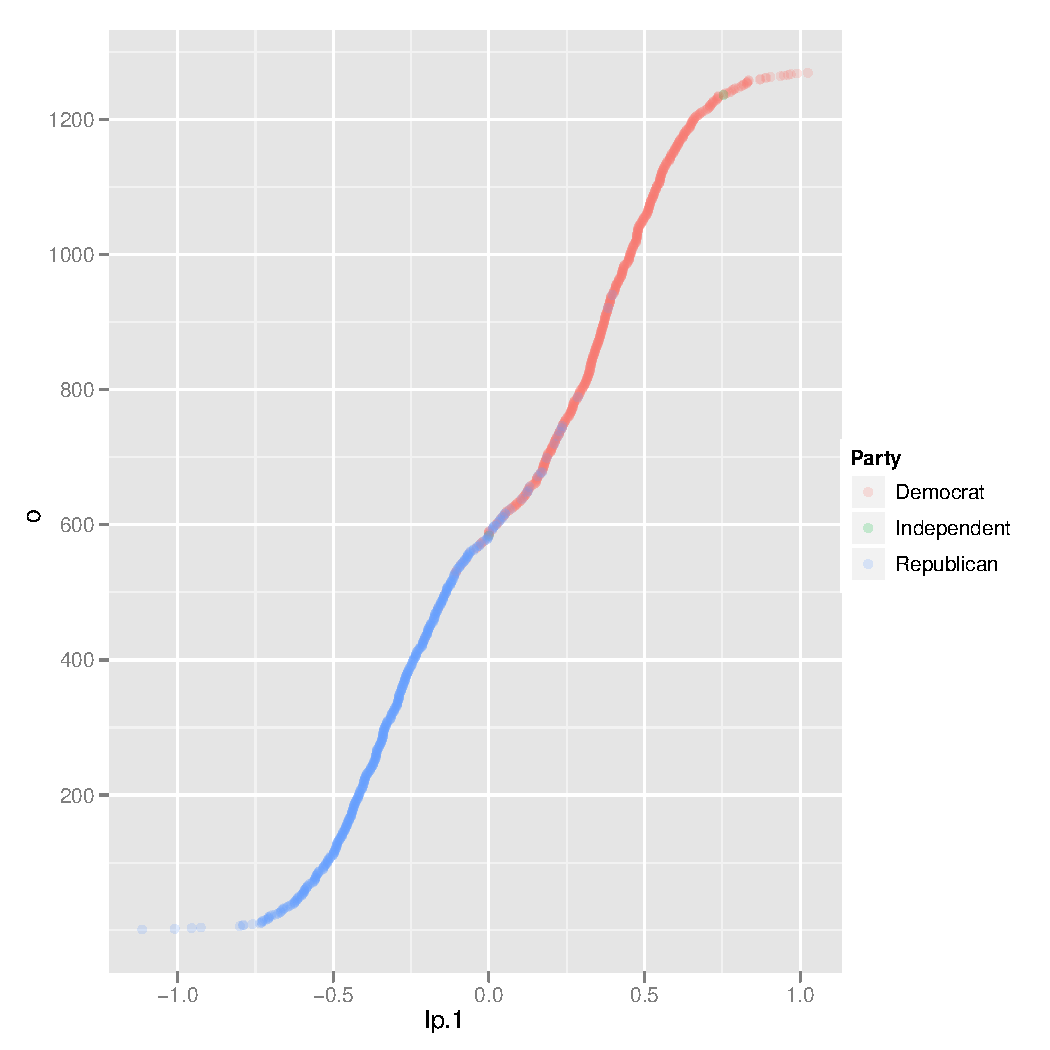
\includegraphics[width=200pt]{figures/legis_src_ip_regression_user_ips.pdf}
  \caption{Legislator ideal points from a 1-dimensional ideal point text regression model.}
  \label{figure:ip_text_regression_ideal_points}
\end{figure}

\paragraph{Semiometrie interpretation}
A particularly nice interpretation of ideal point text regression
comes about when we compare it with semiometrie.  Semiometrie is a
methodology used in marketing and politics for placing users in a
latent space of preferences \cite{camillo:2005}.  To find this latent space, each user $u
\in U$ is asked to provide a rating $r_{ud} \in \{ 1, \ldots, 7 \}$ to
210 words, summarizing their personal warmth toward these words.
Principle component analysis is then applied to the resulting ratings,
optimizing the PCA objective
 \[ \arg \max_{Z \in \mathbb{R}^r, X } \sum_{u \in U, d \in D} \log p(r_{ud} | \bm Z, X),
 \]
where \begin{equation}
\label{equation:rating_draw}
r_{ud} | \bm Z, X \sim N((\bm Z x_u)_d, \sigma_d),
 \end{equation}
 subject to several orthogonalization constraints on $Z$, $X$, and
 $\sigma_d$: they are fit to maximize explained variance.  The
 principle component $\bm z_1 := \bm Z_{1*}$ explains the positive
 ratings shared by everyone: users will share nearly identical
 loadings on this dimension.  We therefore can interpret $\bm z_1$ as an
 intercept column and, for model simplicity, set $x_{*1} = 1$ (we can
 scale the component $\bm z_1$ of $\bm Z$ to do this).  Rewriting
 Equation~\ref{equation:rating_draw} with the intercept $\bm z_1$, we have \[
 r_{ud} | \bm Z, X \sim N((\bm Z_{\setminus1*} x_u + \bm z_1)_d,
 \sigma_d).
 \]

The similarity of ideal point text regression to this scenario is
evident; akin to generalized linear models, we simply replace the
\emph{identity} (normal) link function with the \emph{logit} link
function:
  \[
  \arg \max_{\bm B, \bm b, X} \sum_{u \in U, d \in D} \log p( v_{ud} | \bm B, \bm b, X), \]
where \[ v_{ud} | \bm B, \bm b, X \sim \sigma( \bm w_d^T (\bm B x_u + \bm b) ). \]

In short: the goal of ideal point text regression is to best explain
observed votes by finding an intercept $\bm b$ and subspace $\bm B$
sensitive to user preferences which best explain observed votes.

In semiometrie, the principle component $z_1$ is typically discarded
because it is not informative about individual preferences.  The
intercept $\bm b$ is likewise noninformative about individuals'
preferences, although we keep it to investigate individual words.  At
the same time, the subspace described by $B$ plays the same role as
that of semiometrie: it summarizes legislators by their latent
preferences.